\documentclass[12pt,a4paper]{article}

% Paquetes necesarios
\usepackage[utf8]{inputenc}  % Codificación UTF-8
\usepackage[spanish]{babel}  % Español
\usepackage{amsmath, amssymb, amsthm}  % Paquetes matemáticos
\usepackage{graphicx}  % Para incluir imágenes
\usepackage[margin=1in]{geometry}  % Márgenes
\usepackage{lipsum}  % Texto de ejemplo
\usepackage{float}  % Para usar [H] en figuras
\usepackage{subcaption} % Para usar subfiguras

% Configuración del título
\title{\textbf{Título del Artículo Matemático}}
\author{\textbf{Autor del Artículo}\\ Universidad o Institución}
\date{\today}

\begin{document}

% Portada
\begin{titlepage}
    \centering
    \vspace*{5cm}
    
    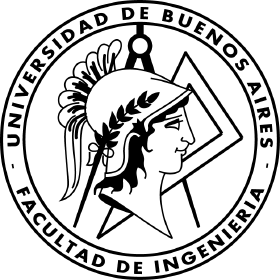
\includegraphics[width=0.4\textwidth]{logo-fiuba.png}\\[1cm]
    
    {\Huge \textbf{Trabajo Práctico 2}}\\[0.2cm]

    {\large \textbf{Aprendizaje Profundo}\\ Alejo Ordoñez}
    
    \vfill
    
    {\large \today}
\end{titlepage}

% Contenido principal
\section*{Resumen}
En este trabajo se abordan el diseño, implementación y análisis de varias arquitecturas de redes neuronales. En particular, se cubren un perceptrón simple, un perceptrón multicapa, una máquina restringuida de Boltzmann, una red convolucional y un autoencoder. Se cubre el algoritmo de aprendizaje gradient descent, usando backpropagation para el cálculo de los gradientes, y se usa el algoritmo de preentrenamiento introducido en el trabajo de Hinton y Salakhutdinov (2006) para la de la máquina de Boltzmann.

\section{Perceptrón simple}
El perceptrón simple es la unidad básica de una red neuronal. Es una neurona artificial que usa una función de activación escalón. La función mapea la entrada $\mathbf{x}$ (un vector de números reales) a una salida binaria $f(\mathbf{x})$:
$$
f(\mathbf{x}) = h (\mathbf{w} \cdot \mathbf{x} + b),
$$
donde $h$ es la función escalón, $\mathbf{w}$ es el vector de pesos, $\mathbf{x}$ es el vector de entradas y $b$ es el sesgo. El sesgo genera una traslación del límite de decisión, que es el hiperplano definido por $\mathbf{w} \cdot \mathbf{x} + b = 0$.
% \begin{figure}[H]
%     \includegraphics[width=0.7\textwidth]{img/perceptrón-simple1.png}
%     \centering
% \end{figure}
El entrenamiento de un perceptrón simple, consiste en la actualizar los pesos y el sesgo de acuerdo a
$$
w_i = \alpha (y - \hat{y}) x_i\\
b = \alpha -(y - \hat{y}),
$$
donde $\alpha$ es la taza de aprendizaje, el par $x, y$ es un ejemplo de entrenamiento y $\hat{y}$ es la salida del perceptrón.
En primer lugar se implementó un perceptrón simple que aprendió la función lógica AND de dos entradas. La tabla de verdad de la función AND es:
% \begin{center}
%     \begin{tabular}{ | c | c | c | c | c |}
%         \hline
%         $x_1$ & $0$ & $0$ & $1$ & $1$\\
%         \hline
%         $x_2$ & $0$ & $1$ & $0$ & $1$\\
%         \hline
%         $\text{AND}(x_1,x_2)$ & $0$ & $0$ & $0$ & $1$\\
%         \hline
%     \end{tabular}
% \end{center}
La evolución del error durante el entrenamiento y la recta discriminadora aprendida por el perceptrón, $x_2 = -(w_1 x_1 = b) / w_2$, se muestran a continuación:
\begin{figure}[H]
  \subcaptionbox*{Evolución del error}[.45\linewidth]{
    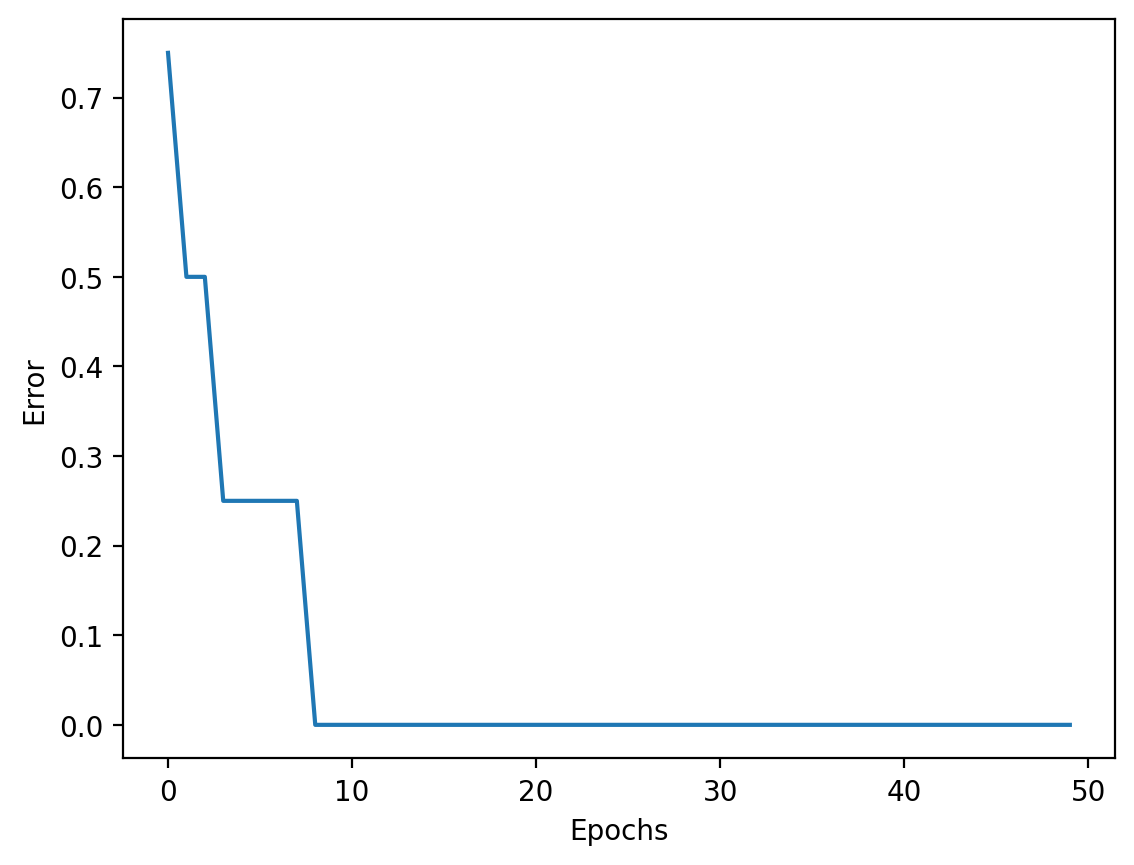
\includegraphics[width=\linewidth]{img/1-training_error.png}
  }
%   \hfill
  \subcaptionbox*{Recta discriminadora}[.45\linewidth]{
    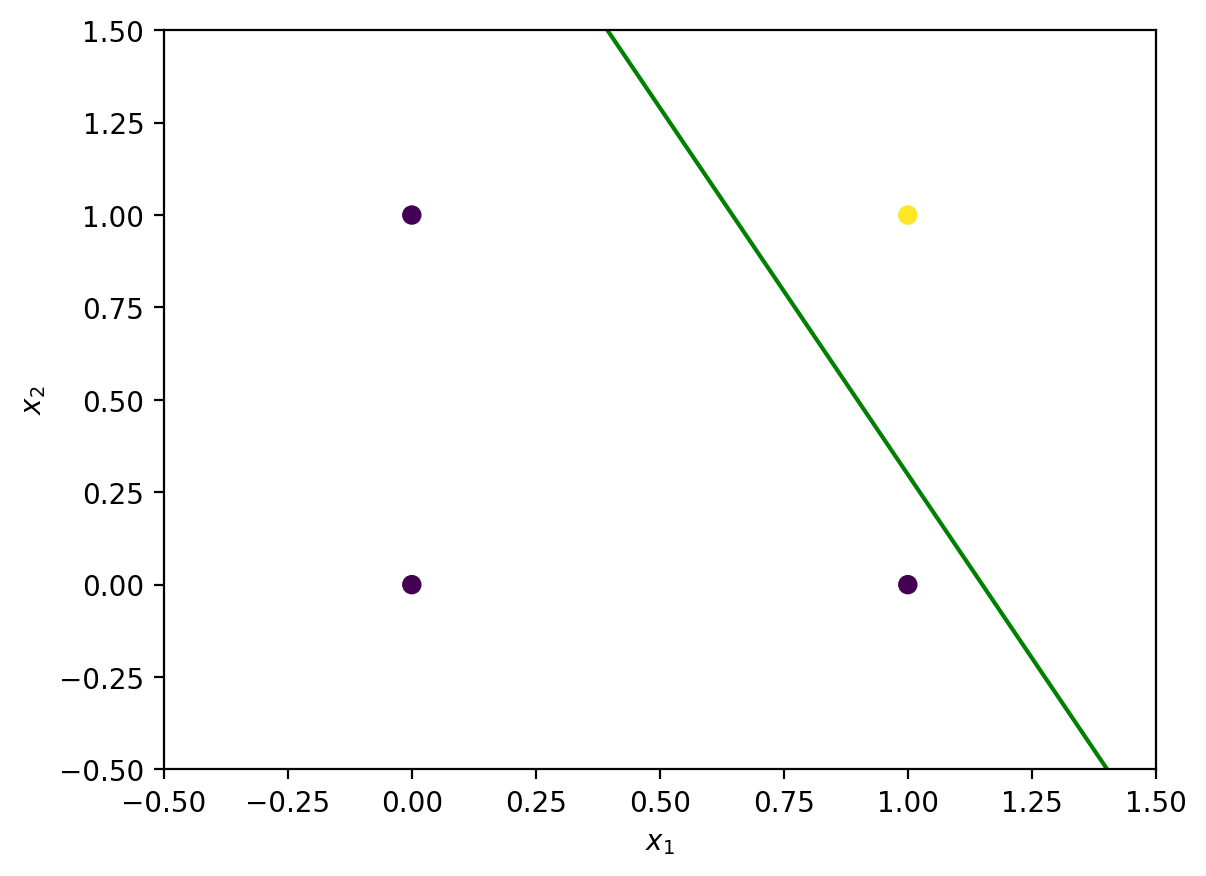
\includegraphics[width=\linewidth]{img/2-desicion_boundary.png}
  }
  \centering
\end{figure}
Seguidamente, se entrenaron perceptrones para que aprendiieran las funciones lógicas OR de dos entradas, y AND y OR de cuatro entradas. Los resultados se muestran a continuación:
\begin{figure}[H]
  \subcaptionbox*{Evolución del error}[.45\linewidth]{
    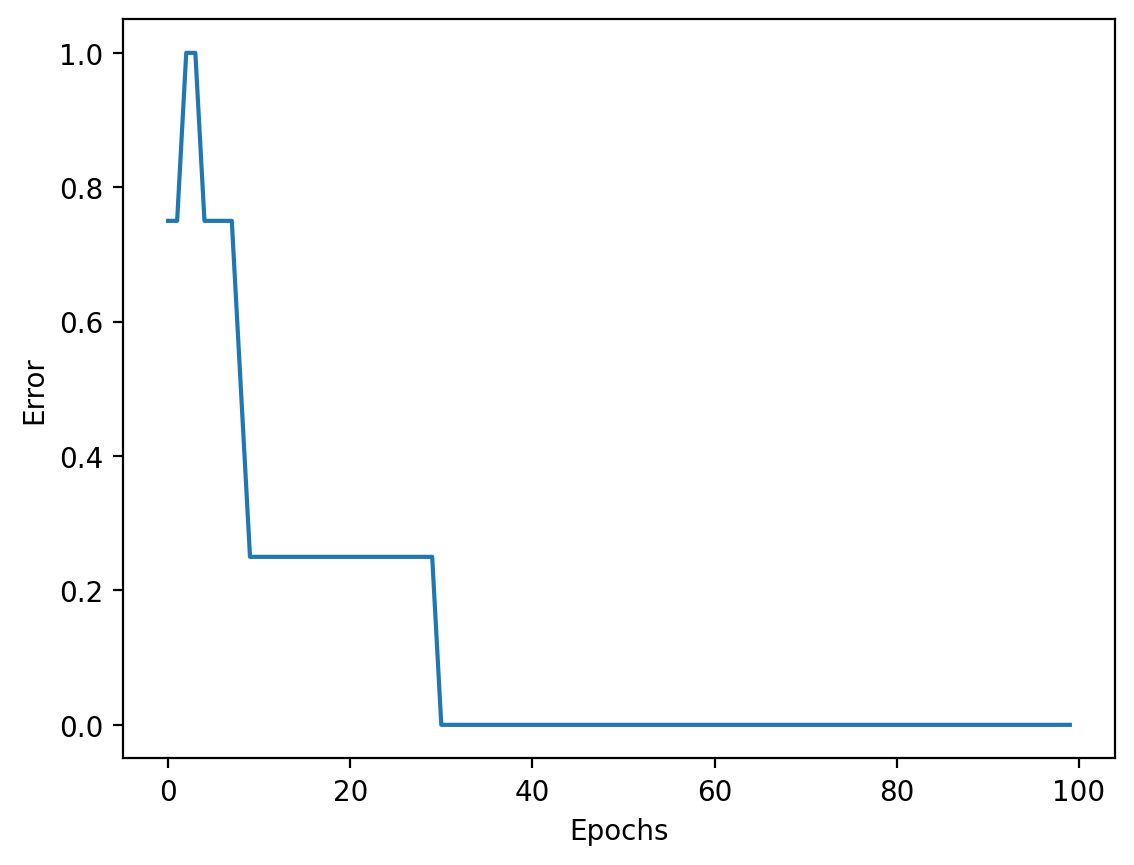
\includegraphics[width=\linewidth]{img/3-training_error.png}
  }
%   \hfill
  \subcaptionbox*{Recta discriminadora}[.45\linewidth]{
    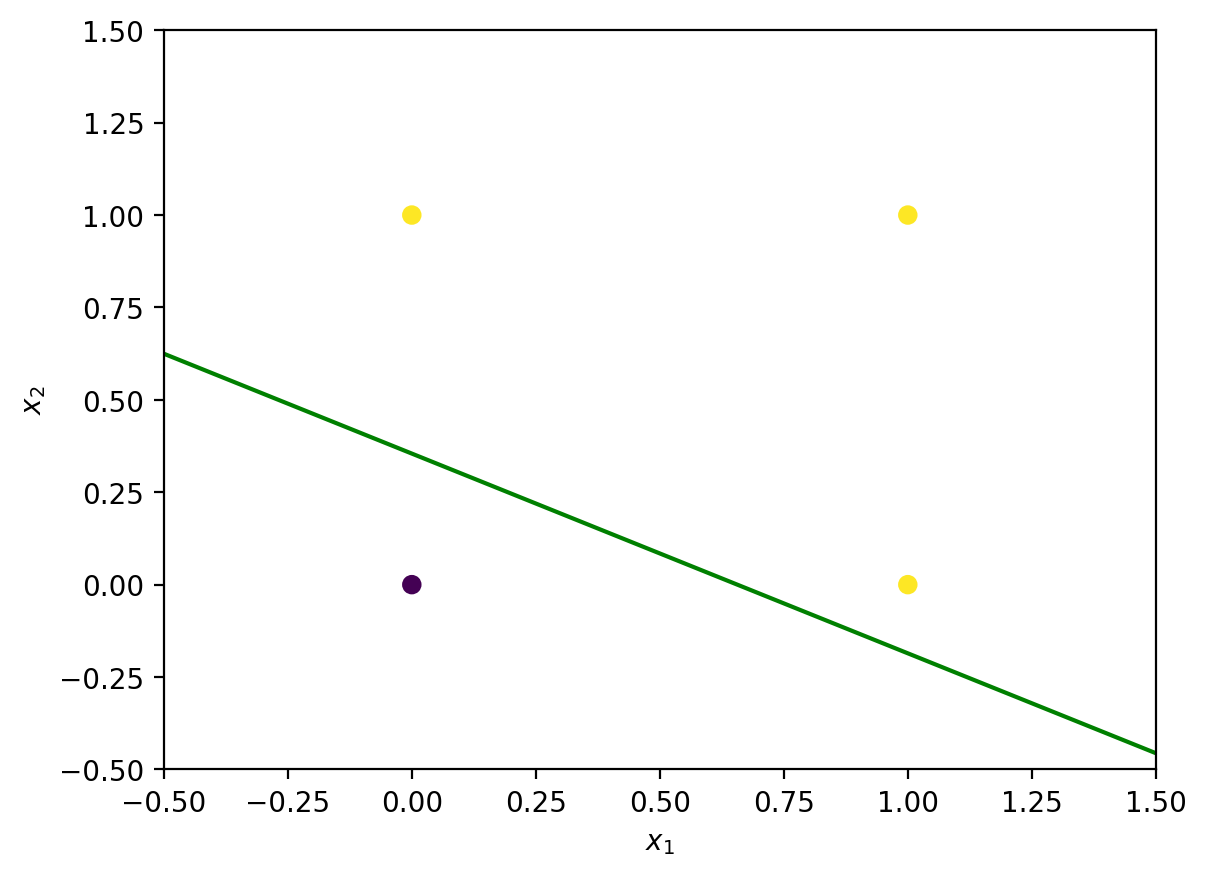
\includegraphics[width=\linewidth]{img/4-desicion_boundary.png}
  }
  \caption{OR de dos entradas}
  \centering
\end{figure}
\begin{figure}[H]
  \subcaptionbox*{AND de cuatro entradas}[.45\linewidth]{
    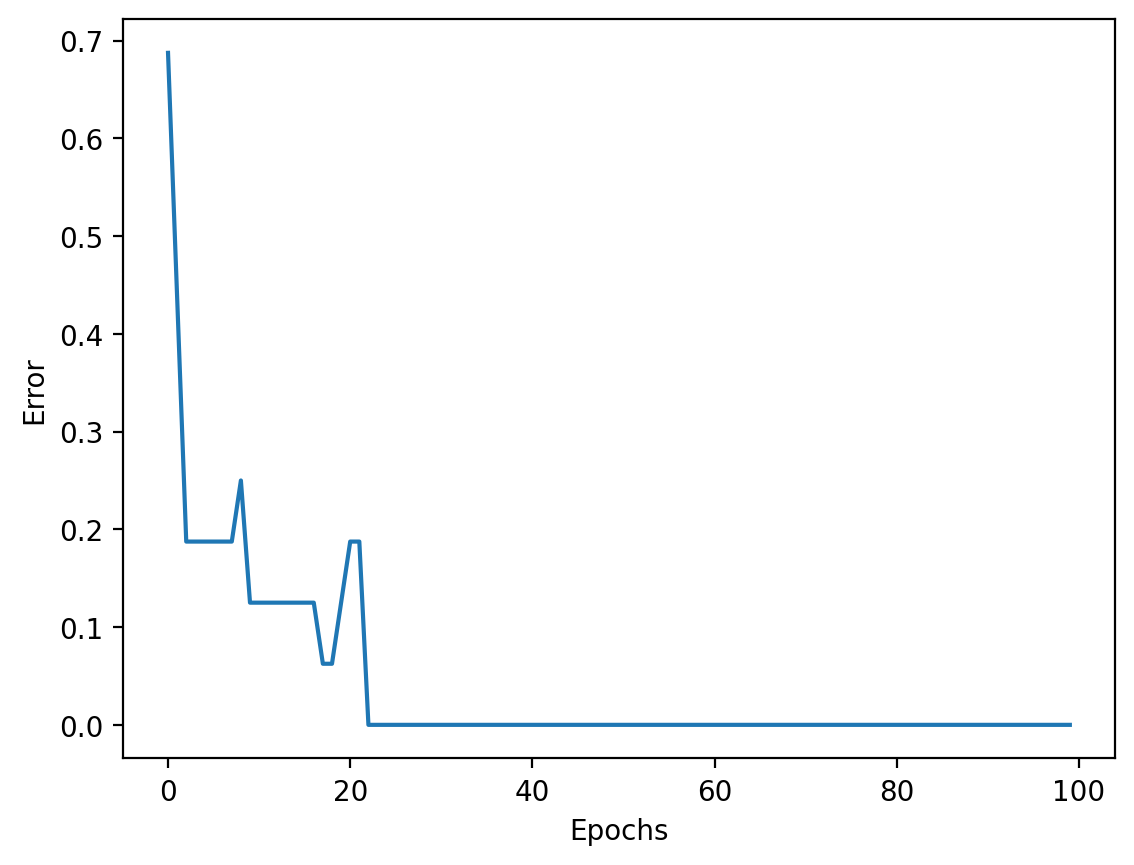
\includegraphics[width=\linewidth]{img/5-training_error.png}
  }
%   \hfill
  \subcaptionbox*{OR de cuatro entradas}[.45\linewidth]{
    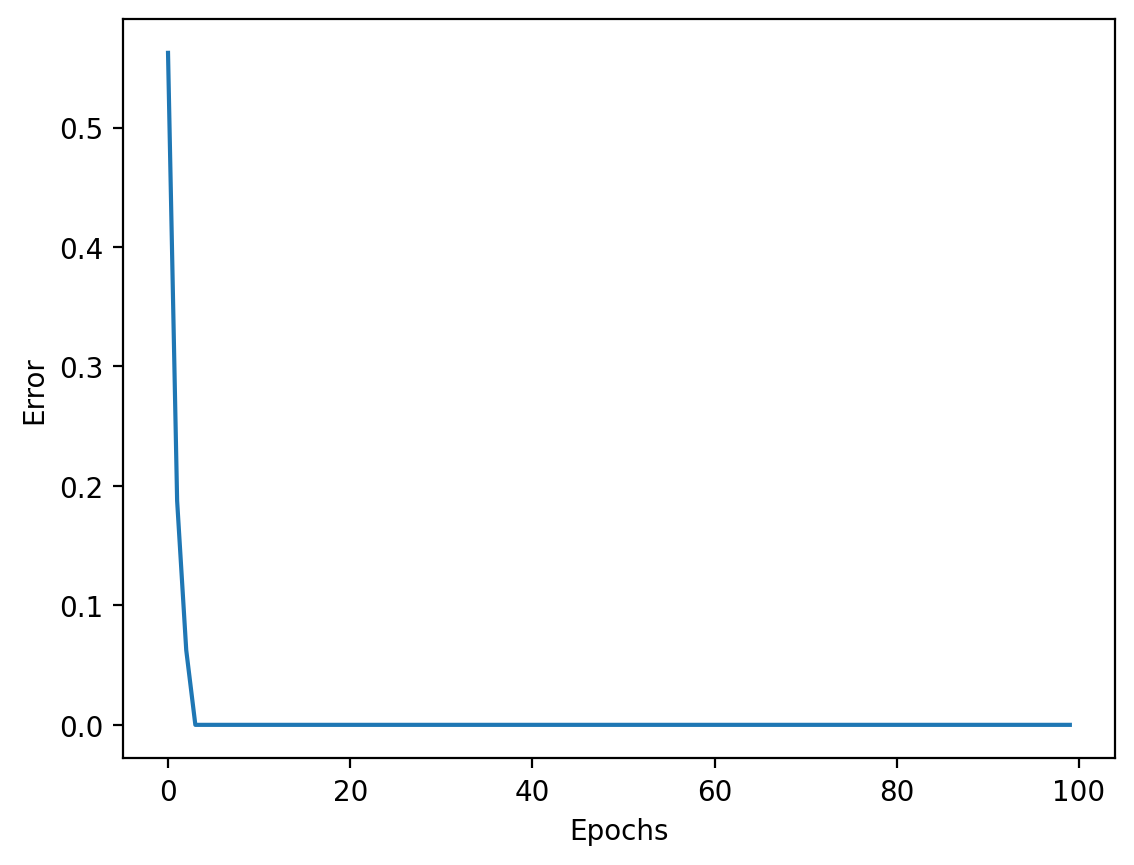
\includegraphics[width=\linewidth]{img/6-training_error.png}
  }
  \caption{Evolución del error}
  \centering
\end{figure}

% Bibliografía
\begin{thebibliography}{9}
% \bibitem{ejemplo} Autor, \emph{Título del libro}, Editorial, Año.
\bibitem{Deep Learning} Ian Goodfellow. Yoshua Bengio. Aaron Courville, \emph{Deep Learning}.
\bibitem{Neural Networks and Deep Learning} Michael Nielsen, \emph{Neural Networks and Deep Learning}.
\bibitem{Reducing the Dimensionality of Data with Neural Networks} G. E. Hinton. R. R. Salakhutdinov, \emph{Reducing the Dimensionality of Data with Neural Networks}.
\bibitem{Object Recognition with Gradient-Based Learning} Yann LeCun. Patrick Haffner. Léon Bottou. Yoshua Bengio, \emph{Object Recognition with Gradient-Based Learning}.

\end{thebibliography}

\end{document}

